\section*{Lezione 7}
\addcontentsline{toc}{section}{Lezione 7}

Kraft da condizione necessaria e sufficiente per fare in modo che esista un codice istantaneo $r$-ario di $q$ simboli avente codeword di lunghezza $\ell_1,\ell_2,...\ell_q$.

MacMillan dimostra che lo \textbf{stesso} teorema è estendibile ai codici univocamente decodificabili.

\begin{figure}[h]
	\centering
	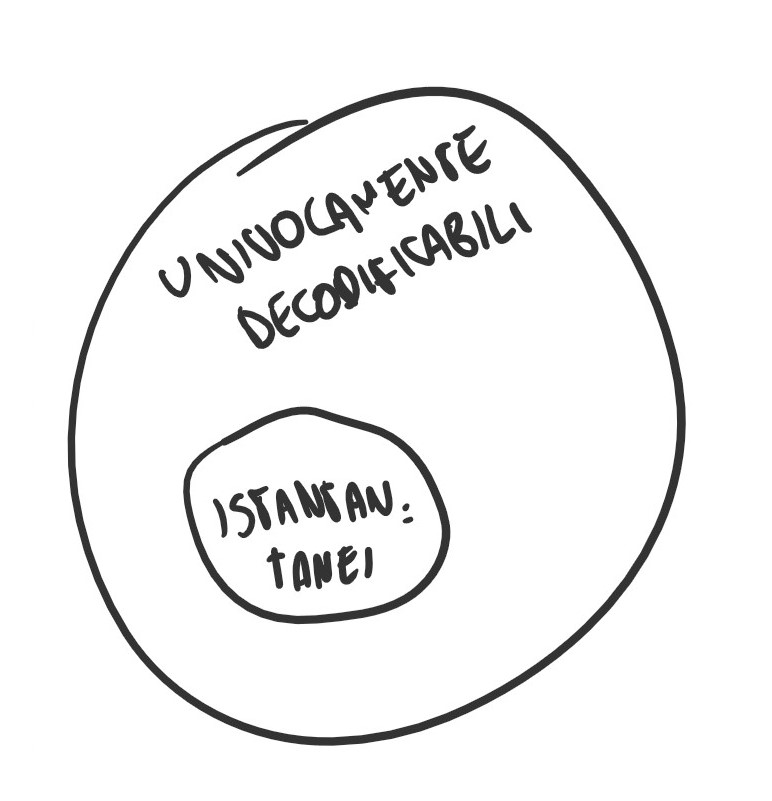
\includegraphics[width=0.5\linewidth]{immagini/img15}
	\caption{I codici istantanei sono un sottoinsieme dei codici univocamente decodificabili}
\end{figure}

\begin{center}
	\large{\textbf{Importante}\\
	$\downarrow$}
\end{center}

\tcbox[tikznode]{Non è vero che \underline{il codice è istantaneo/univocamente decodificabile se $K \leq 1$}\\ ma è vero che \textit{esiste} un codice istantaneo con quelle caratteristiche\\($r$-ario con $q$ caratteri con lunghezze $\ell_1, \ell_2, ... ,\ell_q$) se e solo se $K\leq1$}.

Riprendiamo come esempio questo codice non istantaneo:

\begin{equation*}
s_1 \rightarrow 0
\end{equation*}
\begin{equation*}
s_2 \rightarrow 01
\end{equation*}
\begin{equation*}
s_3 \rightarrow 011
\end{equation*}
\begin{equation*}
s_4 \rightarrow 111
\end{equation*}

Rigirando le cifre codificate:

\begin{equation*}
s_1 \rightarrow 0
\end{equation*}
\begin{equation*}
s_2 \rightarrow 10
\end{equation*}
\begin{equation*}
s_3 \rightarrow 110
\end{equation*}
\begin{equation*}
s_4 \rightarrow 111
\end{equation*}

Otteniamo un codice istantaneo!

Effettivamente la $K$ di Kraft accede solo alle lunghezze delle codeword ($\ell_i$) e il numero di simboli con cui scriviamo le codeword ($r$).\\
Questo per dire che le caratteristiche del codice possono renderlo istantaneo, ma sta poi a chi codifica farlo diventare istantaneo.

\subsection*{Disuguaglianza di McMillan}
\addcontentsline{toc}{subsection}{Disuguaglianza di McMillan}

\begin{theorem}
Condizione necessaria e sufficiente affinchè \textbf{esista} un codice univocamente decodificabile $r$-ario per una sorgente di $q$ simboli con codeword di lunghezze $\ell_1, \ell_2, ... , \ell_q$ è che valga:
\begin{equation}
K=\sum_{i=1}^q\frac{1}{r^{\ell_i}}\leq 1
\end{equation}
\end{theorem}

\begin{enumerate}
	\item Per ogni codice univocamente decodificabile $r$-ario per una sorgente di $q$ simboli con codeword di lunghezze $\ell_1, \ell_2,...,\ell_q$ $\rightarrow K \leq 1$.
	\item Se $K \leq 1$ allora esiste un codice univocamente decodificabile $r$-ario con lunghezze $\ell_1,\ell_2,...,\ell_q$.
\end{enumerate}

\begin{dimostrazione}
Dividiamo l'enunciato del teorema nelle due considerazioni fatte sopra.


\vspace{2mm}
\textbf{Parte 2}:\\
Se $K \leq 1 \rightarrow$ (per Kraft) esiste un codice istantaneo $r$-ario con lunghezze $\ell_1,\ell_2,...,\ell_q$.
Lo stesso codice è univocamente decodificabile (istantaei sono un sottoinsieme di univocamente decodificabili).\\


\vspace{2mm}
\textbf{Parte 1}:\\
Eleviamo $K^n$, dove $n>1$ intero. Quindi avremo che:
\begin{equation*}
K^n=[\sum_{i=1}^{q}\frac{1}{r^{\ell_i}}]^n
\end{equation*}
Definiamo $\ell=max\{\ell_1,\ell_2,...,\ell_q\}$, quindi riscriviamo la sommatoria come:
\begin{equation*}
K^n=\sum_{t=n}^{n\ell}\frac{Nt}{r^{t}}
\end{equation*}
\begin{center}
	N.B. passaggio simile a quello effettuato nella dimostazione della seconda parte di Kraft
\end{center}
Da qui noto che il numeratore $Nt$ è il numero di codeword di lunghezza $t$, ma questo numero non può essere maggiore di $r^t$ visto che rappresenta tutti i possibili vettori lunghi $t$ dove ogni elemento è un carattere dell'alfabeto $r$-ario.
\begin{equation*}
Nt \leq r^t
\end{equation*}
Quindi posso maggiorare la sommatoria:
\begin{equation*}
K^n \leq \sum_{t=n}^{n\ell}\frac{Nt}{r^{t}} = \sum_{t=n}^{n\ell}1 = n\ell-n+1= n\ell-(n-1)
\end{equation*}
$(n-1)$ è negativo visto che per ipotesi $n > 0$, quindi:
\begin{equation*}
K^n \leq n\ell
\end{equation*}
Analizziamo quindi i diversi casi:
\begin{figure}[h]
	\centering
	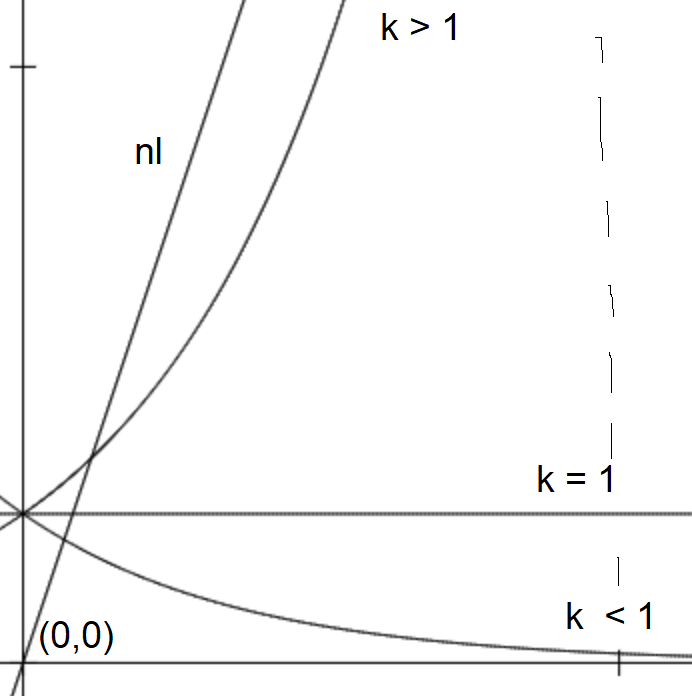
\includegraphics[width=0.5\linewidth]{immagini/img16}
\end{figure}


In maniera asintotica la disuguaglianza è rispettata solo da $k=1$ e $k<1$, quindi questo conclude la dimostazione.
\end{dimostrazione}

Una domanda che potrebbe sorgere è: ha senso utilizzare codici univocamente decodificabili ma non istantanei? No perchè lo sforzo per trovarli è uguali, quindi inutile perderere tempo su codici non istantanei.

Date le probabilità dei simboli qual è il modo più veloce per creare un codice istantaneo che minimizzi $L=\sum_{i=1}^qp_i\ell_i$?

\newpage
\subsection*{Codici a blocchi accorciati}
\addcontentsline{toc}{subsection}{Codici a blocchi accorciati}
Si parte da codeword di lunghezza uguale per poi accorciare.Facciamo un esempio:\\
$r$ = 2\\
$q=5$\\
Per rappresentare 5 simboli ci servono 3 bit; tutte le possibili combinazioni sono:
\begin{center}
	000\\001\\010\\011\\100\\101\\110\\111
\end{center}
Dobbiamo utilizzarne solo 5, quindi scartiamone 3
\begin{center}
	000 $s_1$\\$\cancel{001}$\\010 $s_2$\\$\cancel{011}$\\100 $s_3$\\$\cancel{101}$\\110 $s_4$\\111 $s_5$
\end{center}

A questo punto creiamo un albero di decodifica:

\begin{figure}[H]
	\centering
	\vspace{4mm}
	\begin{tikzpicture}
	[
	grow                    = right,
	level 1/.style={sibling distance=8em},
	level 2/.style={sibling distance=5em},
	level distance          = 7em,
	edge from parent/.style = {draw, -latex},
	every node/.style       = {font=\footnotesize},
	sloped
	]
	\node [root] {}
		child { node [dummy] {}
				child { node [dummy] {}
					child { node [dummy] {$s_5$}
						edge from parent node [above] {1}}
					child { node [dummy] {$s_4$}
						edge from parent node [above] {0}}
					edge from parent node [above] {1}}
				child { node [dummy] {}
					child { node [dummy] {$s_3$}
						edge from parent node [above] {0}}
					edge from parent node [above] {0}}
				edge from parent node [above] {1}}
		child { node [dummy] {}
			child { node [dummy] {}
				child { node [dummy] {$s_2$}
					edge from parent node [above] {0}}
			edge from parent node [above] {1}}
			child { node [dummy] {}
				child { node [dummy] {$s_1$}
					edge from parent node [above] {0}}
				edge from parent node [above] {0}}
			edge from parent node [above] {0}}
	;
	\end{tikzpicture}
	\caption{Albero di decodifica codice a blocchi}
\end{figure}

Partendo dall'albero di questo codice a blocchi, posso effettuare un processo di "sfoltimento" sui nodi di decisione con solo un figlio:

\begin{figure}[H]
	\centering
	\vspace{4mm}
	\begin{tikzpicture}
	[
	grow                    = right,
	level 1/.style={sibling distance=8em},
	level 2/.style={sibling distance=5em},
	level distance          = 7em,
	edge from parent/.style = {draw, -latex},
	every node/.style       = {font=\footnotesize},
	sloped
	]
	\node [root] {}
	child { node [dummy] {}
		child { node [dummy] {}
			child { node [dummy] {$s_5$}
				edge from parent node [above] {1}}
			child { node [dummy] {$s_4$}
				edge from parent node [above] {0}}
			edge from parent node [above] {1}}
		child { node [dummy] {$s_3$}
			edge from parent node [above] {0}}
		edge from parent node [above] {1}}
	child { node [dummy] {}
		child { node [dummy] {$s_2$}
			edge from parent node [above] {1}}
		child { node [dummy] {$s_1$}
			edge from parent node [above] {0}}
		edge from parent node [above] {0}}
	;
	\end{tikzpicture}
	\caption{Albero sfoltito a partire dal precedente}
\end{figure}

Ma come facciamo ad assicurarci che questa sia la migliore codifica per questo problema?

\subsection*{Codici di Huffman}
\addcontentsline{toc}{subsection}{Codici di Huffman}

I codici restituiti dall'algoritmo di Huffman sono \textbf{ottimali}, quindi il valore di $L=\sum_{i=1}^qp_i\ell_i$ è minimo.

Ordiniamo le probabilità dalla più grande alla più piccola (ordine non crescente):

\begin{equation*}
p_1 \geq p_2 \geq ... \geq p_q
\end{equation*}

allora un codice ottimale deve associare queste probabilità alle lunghezze poste in ordine crescente:

\begin{equation*}
\ell_1 \leq \ell_2 \leq ... \leq \ell_q
\end{equation*}

Se questo non è verificato allora il codice non è ottimale.

\begin{dimostrazione}
Assumiamo che le probabiltà siano ordinate in ordine non crescente.\\
Esistono due indici $m$ e $n$ con $m<n$ tali per cui $p_m > p_n$ e $\ell_m > \ell_n$ (quindi viola la regola di prima).
Se questo è vero, posso scambiare le codeword e ottenere una lunghezza media più piccola, quindi il codice iniziale da cui siamo partiti non era ottimale.
Il contributo nella $L$ prima dello scambio era $p_m\ell_m + p_n\ell_n$, questo contributo diventerà $p_m\ell_n+p_n\ell_m$.
La differenza fra queste quantità vale
\begin{equation*}
p_m\ell_n+p_n\ell_m-p_m\ell_m+p_n\ell_n
\end{equation*}
\begin{equation*}
= p_m(\ell_n-\ell_m)-p_n(\ell_n-\ell_m)
\end{equation*}
\begin{equation*}
= (p_m-p_n)(\ell_n-\ell_m)
\end{equation*}
Queste due quantità sono rispettivamente $>0$ e $<0$, quindi la differenza è negativa, quindi scambiando le codeword avrò una lunghezza media minore.
Quindi questo dimostra che sono partito da un codice non ottimale in quanto le lunghezze delle codeword non sono in ordine non decrescente.
\end{dimostrazione}

Ora riconsideriamo

\begin{equation*}
p_1 \geq p_2 \geq ... \geq p_{q-1} \geq p_q
\end{equation*}
\begin{equation*}
\ell_1 \leq \ell_2 \leq ... \leq \ell_{q-1} \leq \ell_q
\end{equation*}

I due simboli meno probabili avranno codeword di uguale lunghezza, per costruzione dell'albero (si apre sempre in due, quindi $\downarrow$)

\begin{figure}[h]
	\centering
	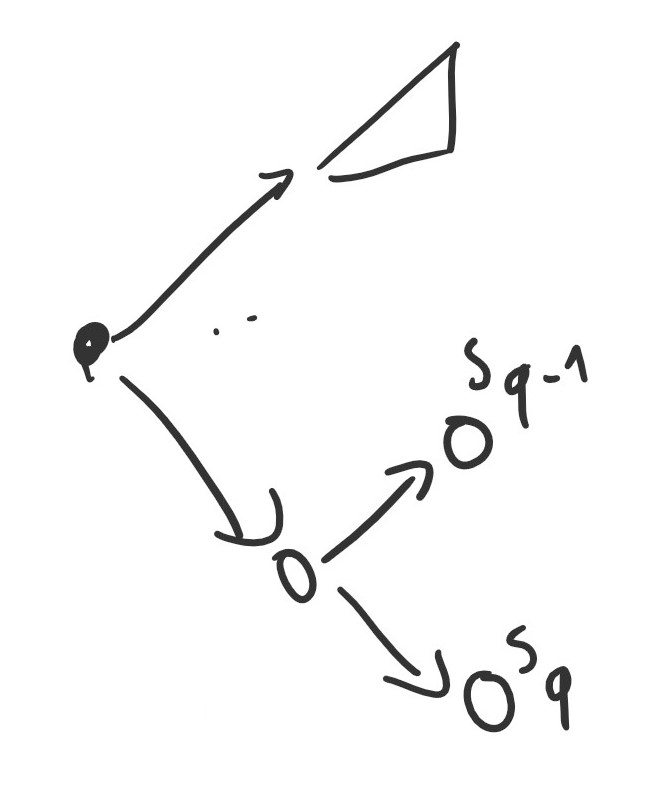
\includegraphics[width=0.3\linewidth]{immagini/img17}
\end{figure}

Quindi per concludere: se le probabilità e le lunghezze seguono la regola precedente e questa regola appena spiegata è rispettata, allora il codice è ottimale.
Ma come creo un codice ottimale?
\newpage
Facciamo un esempio di esecuzione di Algoritmo di Huffman.\\
$r=2$, Abbiamo cinque simboli che escono con le seguenti probabilità:
\begin{center}
	$p_1 = 0.4$\\
	$p_2 = 0.2$\\
	$p_3 = 0.2$\\
	$p_4 = 0.1$\\
	$p_5 = 0.1$
\end{center}
L'algoritmo di Huffman ha un esecuzione di tipo greedy e funziona così:
\begin{enumerate}
\item Prendo i due simboli meno probabili e creo un simbolo 'virtuale' combinandoli, quindi dall'esempio prima otterrò:
\begin{center}
	$p_1 = 0.4$\\
	$p_2 = 0.2$\\
	$p_3 = 0.2$\\
	\hspace{20mm}$p_{4,5} = 0.1 + 0.1=0.2$
\end{center}
\item Itero il passaggio precedente mantenendo traccia delle varie unioni:
\begin{multicols}{3}
	\begin{center}
		$p_1 = 0.4$\\
		$p_2 = 0.2$\\
		$p_3 = 0.2$\\
		$p_{4,5} = 0.2$
	\end{center}
	
	\columnbreak
	
	\begin{center}
		$p_1 = 0.4$\\
		$p_{3,4,5} = 0.4$\\
		$p_2 = 0.2$
	\end{center}  

	\columnbreak
	
	\begin{center}
		$p_1 = 0.4$\\
		$p_{2,3,4,5} = 0.6$
	\end{center}
\end{multicols}
\item Mi fermo quando ottengo $r$ probabilità e assegno un carattere ciascuno:
\begin{center}
	$p_1 = 0.4 \rightarrow \texttt{0}$\\
	$p_{2,3,4,5} = 0.6 \rightarrow \texttt{1}$
\end{center}
\item Ora itero all'indietro, appendendo un carattere alla volta nelle probabilità virtuali (appendo alla fine, se no creo prefissi e il codice non è più istantaneo), quando una virtuale ha lunghezza uguale a un altro simbolo la metto sotto.
\small{
\begin{multicols}{4}
	\begin{center}
		$p_{2,3,4,5} = 0.6 \rightarrow \texttt{0}$
		$p_1 = 0.4 \rightarrow \texttt{1}$\\
	\end{center}
	
	\columnbreak
	
	\begin{center}
		$p_1 = 0.4 \rightarrow \texttt{1}$\\
		$p_{3,4,5} = 0.4 \rightarrow \texttt{00}$
		$p_{2} = 0.2 \rightarrow \texttt{01}$
	\end{center}  
	
	\columnbreak
	
	\begin{center}
		$p_1 = 0.4 \rightarrow \texttt{1}$\\
		$p_{2} = 0.2 \rightarrow \texttt{01}$
		$p_{3} = 0.2 \rightarrow \texttt{000}$
		$p_{4,5} = 0.2 \rightarrow \texttt{001}$
	\end{center}

\columnbreak

\begin{center}
	$p_1 = 0.4 \rightarrow \texttt{1}$\\
	$p_{2} = 0.2 \rightarrow \texttt{01}$
	$p_{3} = 0.2 \rightarrow \texttt{000}$
	$p_{4} = 0.1 \rightarrow \texttt{0010}$
	$p_{5} = 0.1 \rightarrow \texttt{0011}$
\end{center}

\end{multicols}
}
\footnotesize{
Si noti come la regola delle probabilità in ordine inverso rispetto alle lunghezze sia rispettata in tutti i passaggi.
}

\end{enumerate}
Quanto vale la lunghezza media del codice appena calcolato?
\begin{equation*}
L = \sum_{i=1}^qp_i\ell_i = 0.4 \cdot 1 + 0.2 (2+3) + 0.1 \cdot (4+4) = 
\end{equation*}
\begin{equation*}
= 0.4 + 0.2 \cdot 5 + 0.1 \cdot 8 = 0.4 +1+0.8 = 2.2\frac{bit}{simbolo}
\end{equation*}

Proviamo a effettuare un altra esecuzione variando una regola, nel caso due simboli abbiano stessa probabilità, metto sopra quello virtuale (prima era il contrario):
\small{
	\begin{multicols}{4}
		\begin{center}
			$p_1 = 0.4 \rightarrow \texttt{00}$\\
			$p_{2} = 0.2 \rightarrow \texttt{10}$
			$p_{3} = 0.2 \rightarrow \texttt{11}$
			$p_{4} = 0.1 \rightarrow \texttt{010}$
			$p_{5} = 0.1 \rightarrow \texttt{011}$
		\end{center}
		
		\begin{center}
			$p_1 = 0.4 \rightarrow \texttt{00}$\\
			$p_{4,5} = 0.2 \rightarrow \texttt{01}$\\
			$p_{2} = 0.2 \rightarrow \texttt{10}$\\
			$p_{3} = 0.2 \rightarrow \texttt{11}$	
		\end{center}
	
		
		\columnbreak
		
		\begin{center}
			$p_{2,3} = 0.4 \rightarrow \texttt{1}$
			$p_1 = 0.4 \rightarrow \texttt{00}$\\
			$p_{4,5} = 0.2 \rightarrow \texttt{01}$
		\end{center}  
	
		\columnbreak
		
		\begin{center}
			$p_{1,4,5} = 0.6 \rightarrow \texttt{0}$
			$p_{2,3} = 0.4 \rightarrow \texttt{1}$\\
		\end{center}
		
		\columnbreak
	\end{multicols}
}

Le codeword ottenute sono ovviamente diverse, ma la lunghezza media rimarrà uguale:

\begin{equation*}
L = \sum_{i=1}^qp_i\ell_i = 0.4 \cdot 2 + 0.2 (2+2) + 0.1 \cdot (3+3) = 
\end{equation*}
\begin{equation*}
= 0.8 + 0.2 \cdot 4 + 0.1 \cdot 6 = 0.8 +0.8+0.6 = 2.2\frac{bit}{simbolo}
\end{equation*}

Quello che cambia sarà la varianza.





